% This is the template used for the GIH thesis. It is based on 
% Reed College LaTeX thesis template. Most of the work (Reed template)
% for the document class was done by Sam Noble (SN), as well as this
% template. Later comments etc. by Ben Salzberg (BTS). Additional
% restructuring and APA support by Jess Youngberg (JY).
%
% See http://web.reed.edu/cis/help/latex.html for help. There are a
% great bunch of help pages there, with notes on
% getting started, bibtex, etc. Go there and read it if you're not
% already familiar with LaTeX.
%
% Any line that starts with a percent symbol is a comment.
% They won't show up in the document, and are useful for notes
% to yourself and explaining commands.
% Commenting also removes a line from the document;
% very handy for troubleshooting problems. -BTS

% The template was updated by Daniel Hammarström to fit GIH
% requirements. Additional code was borrowed from the 
% Stockholm University (Andreas Solders 2011) template.

% The template was forked from the thesisdown package (CII updates)

%%
%% Preamble
%%
% \documentclass{<something>} must begin each LaTeX document
\documentclass[twoside,10pt]{gihclass} %Default style using S5 paper
% Packages are extensions to the basic LaTeX functions. Whatever you
% want to typeset, there is probably a package out there for it.
% Chemistry (chemtex), screenplays, you name it.
% Check out CTAN to see: http://www.ctan.org/
%%
\usepackage{graphicx,latexsym}
\usepackage{amsmath}
\usepackage{amssymb,amsthm}
\usepackage{longtable,booktabs,setspace}
\usepackage{chemarr} %% Useful for one reaction arrow, useless if you're not a chem major
\usepackage[hyphens]{url}
% Added by CII
\usepackage{hyperref,xcolor}
\hypersetup{
    colorlinks = false,
    pdfborder={0 0 0}
}
\usepackage{lmodern}
\usepackage{float}
\floatplacement{figure}{H}
% End of CII addition
\usepackage{rotating}

% Next line commented out by CII
%%% \usepackage{natbib}
% Comment out the natbib line above and uncomment the following two lines to use the new
% biblatex-chicago style, for Chicago A. Also make some changes at the end where the
% bibliography is included.
%\usepackage{biblatex-chicago}
%\bibliography{thesis}


% Added by CII (Thanks, Hadley!)
% Use ref for internal links
\renewcommand{\hyperref}[2][???]{\autoref{#1}}
\def\chapterautorefname{Chapter}
\def\sectionautorefname{Section}
\def\subsectionautorefname{Subsection}
% End of CII addition

% Added by CII
\usepackage{caption}
\captionsetup{width=5in}
% End of CII addition


% \usepackage{times} % other fonts are available like times, bookman, charter, palatino

% Syntax highlighting #22
  \usepackage{color}
  \usepackage{fancyvrb}
  \newcommand{\VerbBar}{|}
  \newcommand{\VERB}{\Verb[commandchars=\\\{\}]}
  \DefineVerbatimEnvironment{Highlighting}{Verbatim}{commandchars=\\\{\}}
  % Add ',fontsize=\small' for more characters per line
  \usepackage{framed}
  \definecolor{shadecolor}{RGB}{248,248,248}
  \newenvironment{Shaded}{\begin{snugshade}}{\end{snugshade}}
  \newcommand{\AlertTok}[1]{\textcolor[rgb]{0.94,0.16,0.16}{#1}}
  \newcommand{\AnnotationTok}[1]{\textcolor[rgb]{0.56,0.35,0.01}{\textbf{\textit{#1}}}}
  \newcommand{\AttributeTok}[1]{\textcolor[rgb]{0.77,0.63,0.00}{#1}}
  \newcommand{\BaseNTok}[1]{\textcolor[rgb]{0.00,0.00,0.81}{#1}}
  \newcommand{\BuiltInTok}[1]{#1}
  \newcommand{\CharTok}[1]{\textcolor[rgb]{0.31,0.60,0.02}{#1}}
  \newcommand{\CommentTok}[1]{\textcolor[rgb]{0.56,0.35,0.01}{\textit{#1}}}
  \newcommand{\CommentVarTok}[1]{\textcolor[rgb]{0.56,0.35,0.01}{\textbf{\textit{#1}}}}
  \newcommand{\ConstantTok}[1]{\textcolor[rgb]{0.00,0.00,0.00}{#1}}
  \newcommand{\ControlFlowTok}[1]{\textcolor[rgb]{0.13,0.29,0.53}{\textbf{#1}}}
  \newcommand{\DataTypeTok}[1]{\textcolor[rgb]{0.13,0.29,0.53}{#1}}
  \newcommand{\DecValTok}[1]{\textcolor[rgb]{0.00,0.00,0.81}{#1}}
  \newcommand{\DocumentationTok}[1]{\textcolor[rgb]{0.56,0.35,0.01}{\textbf{\textit{#1}}}}
  \newcommand{\ErrorTok}[1]{\textcolor[rgb]{0.64,0.00,0.00}{\textbf{#1}}}
  \newcommand{\ExtensionTok}[1]{#1}
  \newcommand{\FloatTok}[1]{\textcolor[rgb]{0.00,0.00,0.81}{#1}}
  \newcommand{\FunctionTok}[1]{\textcolor[rgb]{0.00,0.00,0.00}{#1}}
  \newcommand{\ImportTok}[1]{#1}
  \newcommand{\InformationTok}[1]{\textcolor[rgb]{0.56,0.35,0.01}{\textbf{\textit{#1}}}}
  \newcommand{\KeywordTok}[1]{\textcolor[rgb]{0.13,0.29,0.53}{\textbf{#1}}}
  \newcommand{\NormalTok}[1]{#1}
  \newcommand{\OperatorTok}[1]{\textcolor[rgb]{0.81,0.36,0.00}{\textbf{#1}}}
  \newcommand{\OtherTok}[1]{\textcolor[rgb]{0.56,0.35,0.01}{#1}}
  \newcommand{\PreprocessorTok}[1]{\textcolor[rgb]{0.56,0.35,0.01}{\textit{#1}}}
  \newcommand{\RegionMarkerTok}[1]{#1}
  \newcommand{\SpecialCharTok}[1]{\textcolor[rgb]{0.00,0.00,0.00}{#1}}
  \newcommand{\SpecialStringTok}[1]{\textcolor[rgb]{0.31,0.60,0.02}{#1}}
  \newcommand{\StringTok}[1]{\textcolor[rgb]{0.31,0.60,0.02}{#1}}
  \newcommand{\VariableTok}[1]{\textcolor[rgb]{0.00,0.00,0.00}{#1}}
  \newcommand{\VerbatimStringTok}[1]{\textcolor[rgb]{0.31,0.60,0.02}{#1}}
  \newcommand{\WarningTok}[1]{\textcolor[rgb]{0.56,0.35,0.01}{\textbf{\textit{#1}}}}

% To pass between YAML and LaTeX the dollar signs are added by CII

% New variables 2019-02-06 GIH copyright info 
\isbn{Provided by the library} 
\place{Stockholm}
\printeby{Printer service, Stockholm, 2019}
\coverinfo{}
\year{2019}



\title{Determinants of intra-individual variation in adaptability to resistance training of different volumes with special reference to skeletal muscle phenotypes}
\author{Daniel Hammarström}
% The month and year that you submit your FINAL draft TO THE LIBRARY (May or December)
\date{May 20xx}


%If you have two advisors for some reason, you can use the following
% Uncommented out by CII
\sernr{999}
% End of CII addition
%%% Remember to use the correct department!

% if you're writing a thesis in an interdisciplinary major,
% uncomment the line below and change the text as appropriate.
% check the Senior Handbook if unsure.
%\thedivisionof{The Established Interdisciplinary Committee for}
% if you want the approval page to say "Approved for the Committee",
% uncomment the next line
%\approvedforthe{Committee}

% Added by CII
%%% Copied from knitr
%% maxwidth is the original width if it's less than linewidth
%% otherwise use linewidth (to make sure the graphics do not exceed the margin)
\makeatletter
\def\maxwidth{ %
  \ifdim\Gin@nat@width>\linewidth
    \linewidth
  \else
    \Gin@nat@width
  \fi
}
\makeatother

\renewcommand{\contentsname}{Table of Contents}
% End of CII addition

\setlength{\parskip}{0pt}

% Added by CII

\providecommand{\tightlist}{%
  \setlength{\itemsep}{0pt}\setlength{\parskip}{0pt}}




\Dedication{
You can have a dedication here if you wish.
}

\Preface{

}

\Abstract{
The preface pretty much says it all.

\par

Second paragraph of abstract starts here.
}

\Listofpapers{
\begin{enumerate}
\def\labelenumi{\Roman{enumi}.}
\item
  \textbf{Hammarström D}, Øfsteng S, Koll L, Hanestadhaugen M, Hollan I, Apró W, Blomstrand E, Rønnestad B, Ellefsen S Benefits of higher resistance-training volume are related to ribosome biogenesis. The \emph{Journal of physiology}. 2020;598(3):543-65.
\item
  Khan Y, \textbf{Hammarström D}, Rønnestad B, Ellefsen S, Ahmad R Increased biological relevance of transcriptome analyses in human skeletal muscle using a model-specific pipeline. \emph{Submitted.}
\item
  \textbf{Hammarström D}, Øfsteng S, Koll L, Jacobsen N, Flobergseter K, Rønnestad B, Ellefsen S Ribosome accumulation during early phase resistance training. \emph{Manuscript}
\item
  \textbf{Hammarström D}, Ellefsen S. generefer: A R package for unbiased selection of reference genes for qPCR in repeated measures designs. \emph{Manuscript}
\end{enumerate}
}


	\usepackage{lettrine} \usepackage{booktabs} \usepackage{longtable} \usepackage{array} \usepackage{multirow} \usepackage{wrapfig} \usepackage{float} \usepackage{colortbl} \usepackage{pdflscape} \usepackage{tabu} \usepackage{threeparttable} \usepackage{threeparttablex} \usepackage[normalem]{ulem} \usepackage{makecell} \usepackage{siunitx}
	\usepackage{booktabs}
\usepackage{longtable}
\usepackage{array}
\usepackage{multirow}
\usepackage{wrapfig}
\usepackage{float}
\usepackage{colortbl}
\usepackage{pdflscape}
\usepackage{tabu}
\usepackage{threeparttable}
\usepackage{threeparttablex}
\usepackage[normalem]{ulem}
\usepackage{makecell}
% End of CII addition
%%
%% End Preamble
%%
%
\begin{document}




% Everything below added by CII


\frontmatter % this stuff will be roman-numbered
% \pagestyle{empty} % this removes page numbers from the frontmatter
  \maketitle
  \begin{dedication}
  \topskip0pt
\vspace*{\fill}
 You can have a dedication here if you wish.
\vspace*{\fill}
  \end{dedication}
\begin{defence}
    THESIS FOR DOCTORAL DEGREE (Ph.D.)\\
    ~\\
    ~\\
    \textbf{The title of your thesis}\\
    ~\\
    by\\
    \textbf{Your name}\\
    ~\\
    ~\\
    Thesis for Philosophy of Doctoral Degree in Sport Sciences, at The Swedish School of Sport and Health Sciences (GIH), which, according to the decision of the dean, will be publicly defended on \emph{DATE}. The thesis defense will be held at the auditorium at The Swedish School of Sport and Health Sciences (GIH), Stockholm.\\
    ~\\
    ~\\
    \textbf{Opponent}\\
    Profesor \ldots.\\
    ~\\
    \textbf{Principal supervisor}\\
    Profesor\ldots{}\\
    ~\\
    \textbf{Co-supervisor(s)}\\
    -Professor\ldots{}\\
    -Professor\ldots{}\\
    -Professor\ldots{}\\
    ~\\
    \textbf{Examination board}\\
    -Associate professor\ldots{}\\
    -Professor \ldots{}\\
    -Professor \ldots{}
  \end{defence}

  \begin{abstract}
    The preface pretty much says it all.
    
    \par
    
    Second paragraph of abstract starts here.
  \end{abstract}
  \begin{listofpapers}
    \begin{enumerate}
    \def\labelenumi{\Roman{enumi}.}
    \item
      \textbf{Hammarström D}, Øfsteng S, Koll L, Hanestadhaugen M, Hollan I, Apró W, Blomstrand E, Rønnestad B, Ellefsen S Benefits of higher resistance-training volume are related to ribosome biogenesis. The \emph{Journal of physiology}. 2020;598(3):543-65.
    \item
      Khan Y, \textbf{Hammarström D}, Rønnestad B, Ellefsen S, Ahmad R Increased biological relevance of transcriptome analyses in human skeletal muscle using a model-specific pipeline. \emph{Submitted.}
    \item
      \textbf{Hammarström D}, Øfsteng S, Koll L, Jacobsen N, Flobergseter K, Rønnestad B, Ellefsen S Ribosome accumulation during early phase resistance training. \emph{Manuscript}
    \item
      \textbf{Hammarström D}, Ellefsen S. generefer: A R package for unbiased selection of reference genes for qPCR in repeated measures designs. \emph{Manuscript}
    \end{enumerate}
  \end{listofpapers}

  \hypersetup{linkcolor=black}
  \setcounter{tocdepth}{2}
  \tableofcontents

  \listoftables

  \listoffigures




\mainmatter % here the regular arabic numbering starts
\pagestyle{fancyplain} % turns page numbering back on

\setcounter{DefaultLines}{3}

\hypertarget{introduction}{%
\chapter{Introduction}\label{introduction}}

\lettrine{S}keletal muscle health is essential for physical independence. In a lifespan perspective, measures of muscle mass and/or strength are inversely associated with mortality
(1--6)
and disability
(7).
Besides adverse associations between of low muscle mass and strength and clinical conditions, muscle weakness also accounts for increased health care costs in patient populations
(8,9).
The intercept between muscle mass, muscle function and health status is interrelated with variables such as age and primary illness or injury
(10).
This highlights that interventions designed to increase muscle mass and strength are likely to prevent adverse health outcomes across the lifespan. A higher level of muscle mass and functional capacity would counteract the effects of muscle loss due to illness, age or inactivity.

Although a large degree of the observed variations in lean mass and strength are attributed to genetic components
(11,12),
environmental factors also contribute, leaving a window of opportunity to increase muscle mass and functional capacity. Among factors affecting muscle mass and functioning are nutrition and pharmacological agents. However, physical activity and specifically systematic resistance training of sufficient volume, intensity and frequency provides a stimulus that promote morphological and functional changes to the human neuromuscular system without adverse side-effects. Irrespective of age, resistance training generally leads to increased muscle mass and strength
(13,14)
and is considered safe when performed in a well organized manner
(14,15).

Resistance training can be modulated indefinitely through combined variations of training variables such as frequency, intensity and volume
(16,17).
Well designed training prescriptions should incorporate information about the current state and goals of the trainee to maximize the potential outcome of the training program
(16--18).
Training volume has received particular attention in the scientific community for many reasons. Evidence suggests that exercise volume affects selected molecular determinants of muscle hypertrophy in a dose-dependent manner
(19--21).
Such effects are believed to facilitate long-term training effects as training programs with higher volume generally result in higher gains in muscle mass and strength with little evidence of differences between age groups or participants with different training backgrounds
(22--24). \\
A consequence of a more extensive training program is the increased time required to complete such a program. As time constraints has been reported as a limiting factor for engaging in physical activity
(25)
some merit can be given to arguments against guidlines suggesting higher volume in resistance training prescription
(18,26).
From an individual perspective, training prescription that balances time-requirement with efficacy presumably increases the likelihood of participation in physical activity (25).
From a more general perspective, increased knowledge about mechanisms governing responses to physical training could improve training prescription also for individuals and populations that experience attenuated benefit of resistance training
(27).
The overreaching goal of the present thesis is to contribute to understanding individualized training loads. To this end, training volume was used to study the effects of variable training stimulus in within-participant models of exercise-training.

\hypertarget{background}{%
\chapter{Background}\label{background}}

\hypertarget{effects-of-resistance-exercise-volume-on-muscle-strength-and-mass}{%
\section{Effects of resistance exercise volume on muscle strength and mass}\label{effects-of-resistance-exercise-volume-on-muscle-strength-and-mass}}

Precise exercise-training\footnote{Exercise is herein defined as an acute bout of physical activity designed to affect physical characteristics such as strength, speed or endurance. Training is defined as the systematic process of combining multiple exercise-sessions performed in sequence over time. Resistance-exercise is defined as an acute strength-promoting program requiring the neuromuscular system to exert force against resistance. Resistance training is defined as a long-term process of multiple resistance exercise-sessions performed over a defined period of time.}
prescription contains information on exercises, their sequential order, intensity and volume at which exercises should be performed, rest periods between efforts or sessions and the frequency at which exercise sessions are to be performed
(23).
By manipulating these variables, resistance training programs can be tailored to better fit goals and starting points of any individual.
The relative importance of exercise-training variables for training outcomes has been examined in numerous studies including (but not limited to) the overall organization of exercise sessions,
({\textbf{???}}, {\textbf{???}})
training frequency
({\textbf{???}},, {\textbf{???}})
and intensity
({\textbf{???}}).
Concerning effects of resistance exercise volume, Berger conducted an early study central to the debate with the goal to determine what method most efficiently produced strength gains (in healthy young males) (28). Berger compared one, two and three sets performed with two, six or ten repetition maximum (RM) in the bench press, three times per week, over twelve weeks. As the combined effect of three sets per session was superior regardless of the number of repetitions performed Berger concluded in favor of three sets. This conclusion was later challenged on the basis of the interpretation of the analysis
(18,26)
Together with additional studies, Carpinelli and Otto instead arrived to the conclusion that there was ``insufficient evidence to support the prevalent belief that a greater volume of exercise (through multiple sets) will elicit superior muscular strength or hypertrophy'' (26). This stand has since been repeatedly put forward as a criticism of higher volume training programs
(29,30) and sparked considerable scientific activity. The main argument against the recommendation of additional volume in strength training programs has been the lack of statistically significant results in single studies (18,29). A second argument against additional volume in strength training recommendation has been the cost/benefit relationship of adding training volume without meaningful additional gains
(18,29).
As benefits of maintaining or increasing functional capacity and muscle mass have been shown to be important for general health
(31)
and sport performance, attempts has been made to synthesize evidence from the literature to challenge the hypothesis that training volume is not important for training induced gains in strength
(22,32)
and muscle mass
(23,24).
The

As acute training variables are inevitably inter-connected, changing one will affect another. Larger exercise volumes per set may for example be achieved when applying lower external resistance. When the total load (repetitions \(\times\) sets \(\times\) external load) is equated by manipulating the external resistance and number of sets greater resistance (and fewer number of sets) leads to similar hypertrophy but higher strength gains
(33).
Higher strength gains are seen as a result of the external resistance ({\textbf{???}})

\hypertarget{the-relationship-between-muscle-mass-and-strength}{%
\section{The relationship between muscle mass and strength}\label{the-relationship-between-muscle-mass-and-strength}}

\hypertarget{meta-analysis-of-exercise-volume}{%
\subsection{Meta-analysis of exercise volume}\label{meta-analysis-of-exercise-volume}}

\hypertarget{molecular-determinants-of-training-induced-muscle-hypertrophy}{%
\section{Molecular determinants of training-induced muscle hypertrophy}\label{molecular-determinants-of-training-induced-muscle-hypertrophy}}

Muscle mass change as a consequence of muscle protein synthesis and breakdown. When a net positive balance is achieved the muscle increase in mass. Resistance exercise leads ta acute blunting of muscle protein synthesis followed by an increase over resting levels in the post exercise period
.

The discovery of an immunosuppressant organic compound called rapamycin in the 1960's led to the characterization of a rapamycin sensitive protein involved in cell growth. The protein was later named mechanistic target for rapamycin (mTOR)
(34). This protein has since been shown play a key role in skeletal muscle hypertrophy in relation to mechanical loading. Bodine \emph{et al.} made a comprehensive characterization of mTOR-mediated skeletal muscle hypertrophy using rodent models in 2001, showing that mTOR activation was essential for load-induced hypertrophy. Additionally, using transfection techniques, they showed that constitutively activated Akt signaling led to hypertrophy in an mTOR-dependent manner, confirmed with concurrent administration of rapamycin (35).
Also in humans, administration of rapamycin, hindering the activity of mTOR leads to an abolished exercise-induced increase in protein synthesis
(36). Furthermore, observational evidence linking mTOR to load-induced hypertrophy comes from human and rodent studies correlating acute phosphorylation the downstream target of mTOR, ribosomal protein S6 kinase (S6K) in response to acute mechanical loading and hypertrophic responses following a subsequent training period
(37,38)

\hypertarget{protein-synthesis}{%
\subsection{Protein synthesis}\label{protein-synthesis}}

Positive net protein balance in responce to exercise

Inhibition of RNA synthesis restrict protein synthesis

Indicated in Goldspink 1977 and 1976 RNA reflects ribosomal availability

Protein synthesis is proportional to RNA content

Increase loading leads to increased RNA
\begin{figure}
\centering
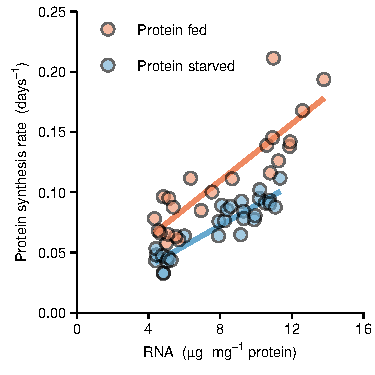
\includegraphics{thesis_files/figure-latex/Millward1973-1.pdf}
\caption{\label{fig:Millward1973}Data from Millward et al.~1973. Group A were fed a diet containing protein, group B were starved or fed a diet not containing protein.}
\end{figure}
\hypertarget{the-mammalian-target-of-rapamycin-mtor-and-translational-efficiency}{%
\subsection{The mammalian target of rapamycin (mTOR) and translational efficiency}\label{the-mammalian-target-of-rapamycin-mtor-and-translational-efficiency}}

The mammalian target of rapamycin (mTOR) is a large serine-threonine protein kinase wich in complex with oyher regulatory proteins forms a signaling hub responsible for responses to environmental cues such as nutrients and mechanical stress.

mTOR has several phosphorylation sites

Phosphorylation of Ser2448 is mediated by S6K1 to reduce mTOR activity in a negative feedback loop .

Ser2448 is phosphorylated by S6K1, changes in nutrient avaliability modifies S6K1 and Ser2448, Ser2448 phosphorylation is abolished when S6K1 is depleted

When the C-terminal is deleted, mTOR gets constitutively active

\hypertarget{ribsome-biogenesisand-muscle-growth}{%
\section{Ribsome biogenesisand muscle growth}\label{ribsome-biogenesisand-muscle-growth}}

Crossland et al.~noted that using IGF-1 induces specific growth related effects in muscle cells. These may be different than the effects induced by sreum as in Stec et al.~

Brook 2016
Stec 2016
Nakada 2016
Figueriedo 2015

Millward 1973 correlation between RNA and protein synthesis

\hypertarget{ribsome-biogenesis}{%
\subsection{Ribsome biogenesis}\label{ribsome-biogenesis}}

\hypertarget{transcription-of-ribsomal-rna-rrna}{%
\subsubsection{Transcription of ribsomal RNA (rRNA)}\label{transcription-of-ribsomal-rna-rrna}}

\hypertarget{transcriptional-activity-related-to-muscle-hypertrophy}{%
\section{Transcriptional activity related to muscle hypertrophy}\label{transcriptional-activity-related-to-muscle-hypertrophy}}

\hypertarget{methods-for-studying-transcriptional-regulation}{%
\subsection{Methods for studying transcriptional regulation}\label{methods-for-studying-transcriptional-regulation}}

\hypertarget{aims}{%
\chapter{Aims}\label{aims}}

The primary aim of this thesis was to relate the adaptive response to resistance training with low- and moderate-volume to skeletal-muscle characteristics in previously untrained individuals. The key question was whether manipulation of exercise-volume will have diverse effects in different individuals related to muscular intrinsic characteristics. A further aim was to characterize exercise-volume dependence and time course profiles of molecular mechanism thought to control resistance training-induced muscle growth. Based on these aims, the objectives of the present thesis were;
\begin{itemize}
\tightlist
\item
  to relate skeletal muscle and systemic characteristics to benefit of moderate- compared to low-volume resistance training;
\item
  To determine volume-dependence in molecular networks related to muscle growth and remodelling in response to mechanical stress
\item
  To determine a time course of markers related to ribosome biogenesis in the early phase of resistance training.
\end{itemize}
\hypertarget{methods}{%
\chapter{Methods}\label{methods}}

\hypertarget{study-participants-protocols-and-training-interventions}{%
\section{Study participants, protocols and training interventions}\label{study-participants-protocols-and-training-interventions}}

Study I was designed to examine effects of low- and moderate-volume on responses to acute exercise and long-term training within participants. Forty-one healthy individuals were recruited and 34 of these completed at least 85\% of the prescribed sessions and were thus included in subsequent data analyses. Reasons for not completing the trial included injury not related to the study (\emph{n =} 1), pain or discomfort during exercises (\emph{n = }5) and non-adherence to the study protocol. There were no differences in characteristics between participants included in or excluded from data analysis in Study I. Study II was designed to study the effects of resistance training \emph{per se} and effects of variable volume on selected markers related to ribosome biogenesis. Participants were therefore recruited to a training group (\emph{n =} 11) and a non-training control group (\emph{n =} 8). Eligible for participation were young (Study I 18-40; Study II 18-35), non-smoking men and women. Exclusion criteria included a training history of more than one weekly session during the last 12 (Study I) or six (Study II) months leading up to the study. Participants were also screened for intolerance to local anesthetic, current or previous injuries affecting their ability to perform resistance training, self-reported symptoms or history of disease, intake of medication or supplements with known effects on adaptations to training. Participant characteristics for both studies are shown in Table \ref{tab:characteristics-table}.
\begin{table}

\caption{\label{tab:characteristics-table}Participant characteristics}
\centering
\fontsize{7}{9}\selectfont
\begin{tabular}[t]{llllllll}
\toprule
  &   & Sex & Age (years) & Stature
(cm) & Mass (kg) & Fat mass (\%) & Lean mass (\%)\\
\midrule
 &  & Female & 22.0 (1.3) & 168 (7) & 64.4 (10.4) & 34.1 (5.6) & 64.3 (6.2)\\
\cmidrule{3-8}
 & \multirow{-2}{*}{\raggedright\arraybackslash Included} & Male & 23.6 (4.1) & 183 (6) & 75.8 (10.7) & 20.4 (6.0) & 79.3 (5.0)\\
\cmidrule{2-8}
 &  & Female & 22.9 (1.6) & 166 (8) & 64.6 (9.7) & 28.8 (8.7) & 68.6 (9.1)\\
\cmidrule{3-8}
\multirow{-4}{*}{\raggedright\arraybackslash Study I} & \multirow{-2}{*}{\raggedright\arraybackslash Excluded} & Male & 24.3 (1.5) & 189 (5) & 88.2 (22.4) & 24.3 (15.3) & 76.8 (12.7)\\
\cmidrule{1-8}
 &  & Female & 23.4 (2.9) & 168 (8) & 64.0 (9.2) & 30.8 (7.1) & 65.5 (6.8)\\
\cmidrule{3-8}
 & \multirow{-2}{*}{\raggedright\arraybackslash Training} & Male & 25.7 (5.8) & 177 (3) & 77.5 (8.0) & 25.3 (3.9) & 71.3 (2.4)\\
\cmidrule{2-8}
 &  & Female & 24.1 (3.5) & 166 (4) & 63.8 (0.6) & 30.5 (6.4) & 66.3 (5.2)\\
\cmidrule{3-8}
\multirow{-4}{*}{\raggedright\arraybackslash Study II} & \multirow{-2}{*}{\raggedright\arraybackslash Control} & Male & 25.5 (5.5) & 182 (5) & 76.5 (7.7) & 18.2 (5.1) & 78.7 (4.2)\\
\bottomrule
\multicolumn{8}{l}{\rule{0pt}{1em}Data are means and (SD)}\\
\end{tabular}
\end{table}
Each training session started with a light standardized warm-up (5 min ergometer cycling and 10 repetitions each of push-ups, sit-ups, back-extensions and squats). Before each exercise in the main program, one set of 10 repetitions were performed in the specific exercise with approximately 50\% of 1RM.

Both studies were fully or partially performed as within-participant studies as each participant had their legs assigned to different training conditions (not including the control group in Study II). Allocation was performed after enrollment where each participant had their legs randomized to either low- or moderate volume (Study I), or variable or constant volume (Study II).

In Study I, the low-volume protocol consisted of a single set of each exercise and the moderate-volume consisted of three sets per exercise. Three unilateral leg exercises were used (leg press, leg curl and knee extension). The moderate volume-leg commenced all sessions and the low volume-leg performed a single set of each exercise in the rest between second and third set of the moderate volume training protocol.

In Study II, only unilateral knee-extension was performed in an effort to concentrate the stimulus to the quadriceps muscles. The constant-volume leg performed six sets of 10RM throughout the study and variable leg performed six sets in session one to four, three sets in session five to eight and nine sets in session nine to twelve with same intensity (10RM).

\hypertarget{ethical-considerations}{%
\subsection{Ethical considerations}\label{ethical-considerations}}

Both studies were approved by the local ethics committee Lillehammer University College/Inland Norway University of Applied Sciences and the Norwegian Centre for Research Data. In accordance with the \emph{Declaration of Helsinki}(39) the studies were pre-registered in publicly accessible databases (Study I, ClinicalTrials.gov Identifier: NCT02179307; Study II, \url{https://osf.io/wa96y}). Participants were informed of the study design, potential risks and sources of discomfort prior to giving their informed consent.

\hypertarget{measures-of-muscle-mass}{%
\section{Measures of muscle mass}\label{measures-of-muscle-mass}}

In Study I muscle mass was measured by magnetic resonance imaging (MRI) and dual energy X-ray absorptiometry (DXA) prior to and after the intervention. Both MRI and DXA measurements were completed during the same visit to the laboratory. Participants were instructed to refrain from strenuous physical activity during the last 48 h leading up to the measurements. The post-training measurements were completed at least 48 h after the last strength testing session. Participants were asked to refrain from food consumption during 2 h leading up to the measurements.

MRI images were obtained from the mid-thigh and analyzed by the same investigator blinded for time (pre- and post-training) and condition (low- and moderate-volume). Multiple images were used to estimate the cross-sectional area of the extensor muscles at the same distance from the knee-joint.

See figure

Dallin et al.~recently estimated the (40)

\hypertarget{muscle-strength-assessments}{%
\section{Muscle strength assessments}\label{muscle-strength-assessments}}

Muscle strength was with

\hypertarget{blood-variables}{%
\section{Blood variables}\label{blood-variables}}

\hypertarget{muscle-tissue-sampling-and-preparations-for-downstream-analyses}{%
\section{Muscle tissue sampling and preparations for downstream analyses}\label{muscle-tissue-sampling-and-preparations-for-downstream-analyses}}

Muscle samples were obtained under local anesthesia (Study I, Xylocaine, \SI{10}{\mg\per\ml} with adrenalin \SI{5}{\micro\gram\per\ml}, AstraZeneca, Oslo, Norway; Study II, Lidocaine Mylan, \SI{10}{\mg\per\ml}, Mylan Ireland Ltd, Ireland) with a fine needle (12-14 gauge; Universal-plus, Medax, Italy) operated with a spring-loaded instrument (Bard Magnum, Bard Norway AS, Norway). Sampling was performed as previously described
(41),
with modifications. Anestheisa was injected in the subcutanous tissue with care taken not to inject anesthesia into the muscle itself. Following a short period (5 min) the effect of the anesthesia was confirmed using an injection needle. Following pilot experiments we decided not to use an insertion cannula as described in (41) as the biopsy needle itself could be used to puncture the skin and muscle fascia. This also resulted in less discomfort. Several passes through the same skin puncture was made to obtain sufficient material for downstream analyses. A smaller needle (14 vs.~12 gauge) was used to further minimized discomfort in Study II where more biopsies were sampled over a shorter time span, with exception from when material was used for immunhistochemistry. The first biopsy was sampled at one third of the distance between the patella to the \emph{anterior superior iliac spinae} with subsequent biopsies sampled \(\sim\)\SI{2}{cm} proximal to previous samples. In Study II samples obtained more than one week apart were sampled with closer proximity and distally from previous samples but never at previous sampling sites.

The microbiopsy technique produces smaller samples compared to other biopsy techniques
(42), and thus requires several passes to produce sufficient material for multiple downstream experiments. However, reports confirms that the microbiopsy technique is comparable to the traditionally used Bergström technique in several measures of muscle characteristics at the same time as being well tolerated
(41,43).
Any reported differences in fiber type distributions between sampling techniques have been suggested relating to differences in sampling depth
(43,44). \\
For determination of fiber type distributions, a threshold of 200-300 fibers has been suggested as a suitable sample size per specimen as more fibers does not reduce the variation between dupliacte samples
(45).
In Study I one or several pieces of muscle (total weight \(\sim\)\SI{15}{mg}) were chosen per sampling for analysis of fiber type distributions (described in detail below). The total number of fibers were counted from these specimens (Figure ref fig). Using an average of fibers from the first sampling time point the between leg coefficient of variation was determined to 14\% for Type I fibers and 11.3 for type II fibers. The between leg variation in Type I fibers is similar to what has been previously reported {[}Blomstrand Ekblom{]}

Latest paper on variability between samples from the same leg and due to number of fibers counted
Appl Physiol Nutr Metab
. 2020 Apr;45(4):368-375. doi: 10.1139/apnm-2019-0263. Epub 2020 Mar 24.

The within-leg was similar to between leg comparison in our samples. This might highlight sampling depth variation in microbiopsy technique in immunohistochemistry ?

To calculate variation in proportions

\url{https://www.ncbi.nlm.nih.gov/pmc/articles/PMC3875499/}
\begin{verbatim}
Using ',' as decimal and '.' as grouping mark. Use read_delim() for more control.
\end{verbatim}
\begin{verbatim}
Parsed with column specification:
cols(
  subject = col_character(),
  multiple = col_character(),
  single = col_character(),
  sex = col_character(),
  include = col_character()
)
\end{verbatim}
\begin{verbatim}
Joining, by = c("subject", "leg")
Joining, by = c("subject", "leg")
Joining, by = c("subject", "leg")
\end{verbatim}
\begin{figure}

{\centering 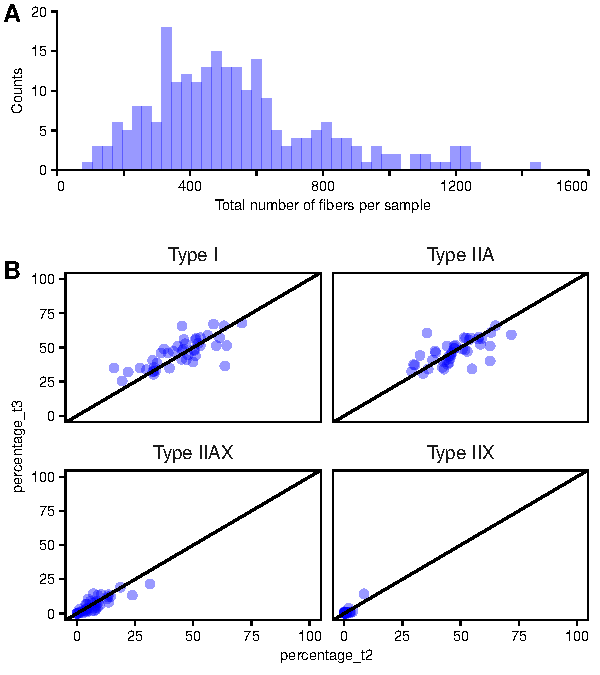
\includegraphics{thesis_files/figure-latex/immuno-methods-1} 

}

\caption[Fiber counts]{Number of fibres in immunohistochemistry analyses}\label{fig:immuno-methods}
\end{figure}
\hypertarget{gene-expression-analysis}{%
\section{Gene expression analysis}\label{gene-expression-analysis}}

\hypertarget{determination-of-protein-abundance}{%
\section{Determination of protein abundance}\label{determination-of-protein-abundance}}

\hypertarget{statistics-and-data-analysis}{%
\section{Statistics and data analysis}\label{statistics-and-data-analysis}}

TO DO:
\begin{itemize}
\tightlist
\item
  For methods discussion, compare product length, efficiencies and ct values in relation to RQI-values. See Fleige 2006 for reference.
\end{itemize}
\hypertarget{gene-expression-analysis-1}{%
\section{Gene expression analysis}\label{gene-expression-analysis-1}}

\hypertarget{normalization}{%
\subsection{Normalization}\label{normalization}}
\begin{itemize}
\tightlist
\item
  An external reference gene was added at a constant amount in Trizol preps
\item
  A normalization factor was used to express relative target gene abundance per-weight tissue.
\item
  In qPCR the linearised expression (effectivety \^{}cq) was used to express the fraction of external reference per total RNA.
\item
  In RNA-seq the external reference gene was sequenced and counts were used to express external RNA as a fraction of total RNA.
\item
  In both cases the normalization factor was calculated as mw * counts.
\end{itemize}
A simulation to see that this is equivalent to tissue used in prep when no measurement errors exists.
\begin{Shaded}
\begin{Highlighting}[]
\KeywordTok{library}\NormalTok{(tidyverse)}

\KeywordTok{expand_grid}\NormalTok{(}\DataTypeTok{mg =} \KeywordTok{seq}\NormalTok{(}\DataTypeTok{from =} \DecValTok{5}\NormalTok{, }\DataTypeTok{to =} \DecValTok{100}\NormalTok{, }\DataTypeTok{by =} \DecValTok{5}\NormalTok{), }
            \DataTypeTok{rna.mg =} \KeywordTok{seq}\NormalTok{(}\DataTypeTok{from =} \DecValTok{250}\NormalTok{, }\DataTypeTok{to =} \DecValTok{600}\NormalTok{, }\DataTypeTok{by =} \DecValTok{25}\NormalTok{),}
            \DataTypeTok{ext =} \FloatTok{0.04}\NormalTok{) }\OperatorTok
\StringTok{  }\KeywordTok{mutate}\NormalTok{(}\DataTypeTok{tot.rna =}\NormalTok{ mg }\OperatorTok{*}\StringTok{ }\NormalTok{rna.mg, }
         \DataTypeTok{ext.frac =}\NormalTok{ ext }\OperatorTok{/}\StringTok{ }\NormalTok{(ext }\OperatorTok{+}\StringTok{ }\NormalTok{tot.rna), }
         \DataTypeTok{mg.inprep =} \DecValTok{1000} \OperatorTok{/}\StringTok{ }\NormalTok{((ext }\OperatorTok{+}\StringTok{ }\NormalTok{tot.rna) }\OperatorTok{/}\StringTok{ }\NormalTok{mg), }
         \DataTypeTok{nf =}\NormalTok{ ext.frac }\OperatorTok{*}\StringTok{ }\NormalTok{mg) }
\end{Highlighting}
\end{Shaded}
\begin{verbatim}
# A tibble: 300 x 7
      mg rna.mg   ext tot.rna  ext.frac mg.inprep        nf
   <dbl>  <dbl> <dbl>   <dbl>     <dbl>     <dbl>     <dbl>
 1     5    250  0.04    1250 0.0000320      4.00 0.000160 
 2     5    275  0.04    1375 0.0000291      3.64 0.000145 
 3     5    300  0.04    1500 0.0000267      3.33 0.000133 
 4     5    325  0.04    1625 0.0000246      3.08 0.000123 
 5     5    350  0.04    1750 0.0000229      2.86 0.000114 
 6     5    375  0.04    1875 0.0000213      2.67 0.000107 
 7     5    400  0.04    2000 0.0000200      2.50 0.000100 
 8     5    425  0.04    2125 0.0000188      2.35 0.0000941
 9     5    450  0.04    2250 0.0000178      2.22 0.0000889
10     5    475  0.04    2375 0.0000168      2.11 0.0000842
# ... with 290 more rows
\end{verbatim}
\begin{Shaded}
\begin{Highlighting}[]
\KeywordTok{expand_grid}\NormalTok{(}\DataTypeTok{mg =} \KeywordTok{seq}\NormalTok{(}\DataTypeTok{from =} \DecValTok{5}\NormalTok{, }\DataTypeTok{to =} \DecValTok{100}\NormalTok{, }\DataTypeTok{by =} \DecValTok{5}\NormalTok{), }
            \DataTypeTok{rna.mg =} \KeywordTok{seq}\NormalTok{(}\DataTypeTok{from =} \DecValTok{50}\NormalTok{, }\DataTypeTok{to =} \DecValTok{600}\NormalTok{, }\DataTypeTok{by =} \DecValTok{25}\NormalTok{),}
            \DataTypeTok{ext =} \FloatTok{0.04}\NormalTok{) }\OperatorTok
\StringTok{  }\KeywordTok{mutate}\NormalTok{(}\DataTypeTok{tot.rna =}\NormalTok{ mg }\OperatorTok{*}\StringTok{ }\NormalTok{rna.mg, }
         \DataTypeTok{ext.frac =}\NormalTok{ ext }\OperatorTok{/}\StringTok{ }\NormalTok{(ext }\OperatorTok{+}\StringTok{ }\NormalTok{tot.rna), }
         \DataTypeTok{mg.inprep =} \DecValTok{1000} \OperatorTok{/}\StringTok{ }\NormalTok{((ext }\OperatorTok{+}\StringTok{ }\NormalTok{tot.rna) }\OperatorTok{/}\StringTok{ }\NormalTok{mg), }
         \DataTypeTok{nf =}\NormalTok{ ext.frac }\OperatorTok{*}\StringTok{ }\NormalTok{mg) }\OperatorTok
\StringTok{         }\KeywordTok{ggplot}\NormalTok{(}\KeywordTok{aes}\NormalTok{(rna.mg, mg.inprep,  }\DataTypeTok{color =}\NormalTok{ mg)) }\OperatorTok{+}\StringTok{ }\KeywordTok{geom_point}\NormalTok{(}\DataTypeTok{size =} \DecValTok{2}\NormalTok{)}
\end{Highlighting}
\end{Shaded}
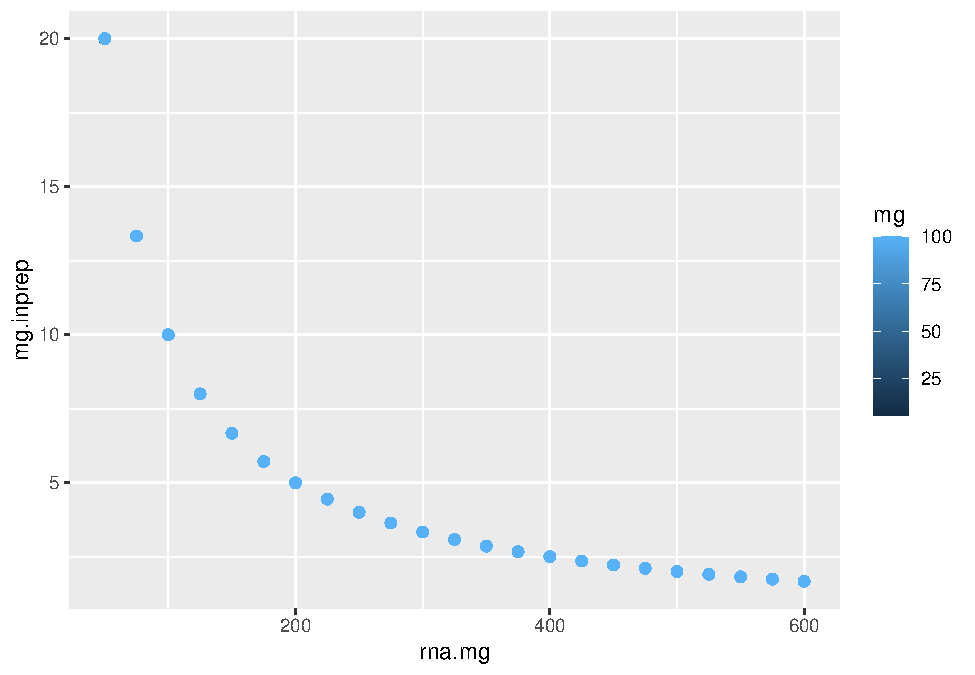
\includegraphics{thesis_files/figure-latex/unnamed-chunk-1-1.pdf}

\hypertarget{training-protocols}{%
\section{Training protocols}\label{training-protocols}}

A full body protocol was used in study I including

\hypertarget{results-and-discussion}{%
\chapter{Results and Discussion}\label{results-and-discussion}}

\hypertarget{effects-of-different-training-volume-on-changes-in-muscle-size-and-function}{%
\section{Effects of different training volume on changes in muscle size and function}\label{effects-of-different-training-volume-on-changes-in-muscle-size-and-function}}

In Study I, the average increases (Table \ref{tab:csa-str-tab}) in muscle strength and mass in each volume condition corresponded to what could be expected based on previous studies
(13,46).




\begin{table}

\caption{\label{tab:csa-str-tab}Training induced changes in muscle CSA and average strength in Study I}
\centering
\fontsize{7}{9}\selectfont
\begin{tabular}[t]{lllll}
\toprule
 & Sex & Volume condition & Mean (SD) & Reference\\
\midrule
 &  & LOW & 3.05 (3.61) & \\
\cmidrule{3-4}
 & \multirow{-2}{*}{\raggedright\arraybackslash Female} & MOD & 5.02 (4.04) & \\
\cmidrule{2-4}
 &  & LOW & 3.83 (3.50) & \\
\cmidrule{3-4}
\multirow{-4}{*}{\raggedright\arraybackslash CSA \%-change} & \multirow{-2}{*}{\raggedright\arraybackslash Male} & MOD & 5.10 (3.71) & \multirow{-4}{*}{\raggedright\arraybackslash }\\
\cmidrule{1-5}
 &  & LOW & 0.04 (0.05) & \\
\cmidrule{3-4}
 & \multirow{-2}{*}{\raggedright\arraybackslash Female} & MOD & 0.07 (0.05) & \\
\cmidrule{2-4}
 &  & LOW & 0.05 (0.05) & \\
\cmidrule{3-4}
\multirow{-4}{*}{\raggedright\arraybackslash CSA \%-change day} & \multirow{-2}{*}{\raggedright\arraybackslash Male} & MOD & 0.07 (0.05) & \multirow{-4}{*}{\raggedright\arraybackslash 0.11 [0.04-0.26]a}\\
\cmidrule{1-5}
 &  & LOW & 0.11 (0.13) & \\
\cmidrule{3-4}
 & \multirow{-2}{*}{\raggedright\arraybackslash Female} & MOD & 0.18 (0.15) & \multirow{-2}{*}{\raggedright\arraybackslash 0.08 (0.22)b}\\
\cmidrule{2-5}
 &  & LOW & 0.14 (0.12) & \\
\cmidrule{3-4}
\multirow{-4}{*}{\raggedright\arraybackslash CSA \%-change session} & \multirow{-2}{*}{\raggedright\arraybackslash Male} & MOD & 0.19 (0.13) & \multirow{-2}{*}{\raggedright\arraybackslash 0.14 (0.14)b}\\
\cmidrule{1-5}
 &  & LOW & 21.0 (9.8) & \\
\cmidrule{3-4}
 & \multirow{-2}{*}{\raggedright\arraybackslash Female} & MOD & 27.8 (14.4) & \\
\cmidrule{2-4}
 &  & LOW & 19.2 (12.4) & \\
\cmidrule{3-4}
\multirow{-4}{*}{\raggedright\arraybackslash Average strength \%-change} & \multirow{-2}{*}{\raggedright\arraybackslash Male} & MOD & 23.1 (12.0) & \multirow{-4}{*}{\raggedright\arraybackslash }\\
\cmidrule{1-5}
 &  & LOW & 0.77 (0.36) & \\
\cmidrule{3-4}
 & \multirow{-2}{*}{\raggedright\arraybackslash Female} & MOD & 1.00 (0.49) & \multirow{-2}{*}{\raggedright\arraybackslash 0.67 (0.35)b}\\
\cmidrule{2-5}
 &  & LOW & 0.72 (0.48) & \\
\cmidrule{3-4}
\multirow{-4}{*}{\raggedright\arraybackslash Average strength \%-session} & \multirow{-2}{*}{\raggedright\arraybackslash Male} & MOD & 0.87 (0.46) & \multirow{-2}{*}{\raggedright\arraybackslash 0.47 (0.22)b}\\
\bottomrule
\multicolumn{5}{l}{\textsuperscript{a} Estimates from Wernbom et al. (46)}\\
\multicolumn{5}{l}{\textsuperscript{b} Estimates from Ahtiainen et al. (ref:ahtiainen-citation}\\
\end{tabular}
\end{table}
Average within participant differences in responses between LOW and MOD were consistent across measures of muscle hypertrophy and strength gains (Figure \ref{fig:comb-fig-s1}). These differences were in agreement to what could be expected based on published meta-analyses
(22--24,32).
Taken together, these observations confirmed the efficacy of the training program in general and a dose-response with regard to within-session exercise volume.

In Study II, training efficacy was assessed by comparing outcomes to a non-training control group. The training group displayed increases compared to the control group for both strength muscle thickness measures.
\begin{figure}

{\centering 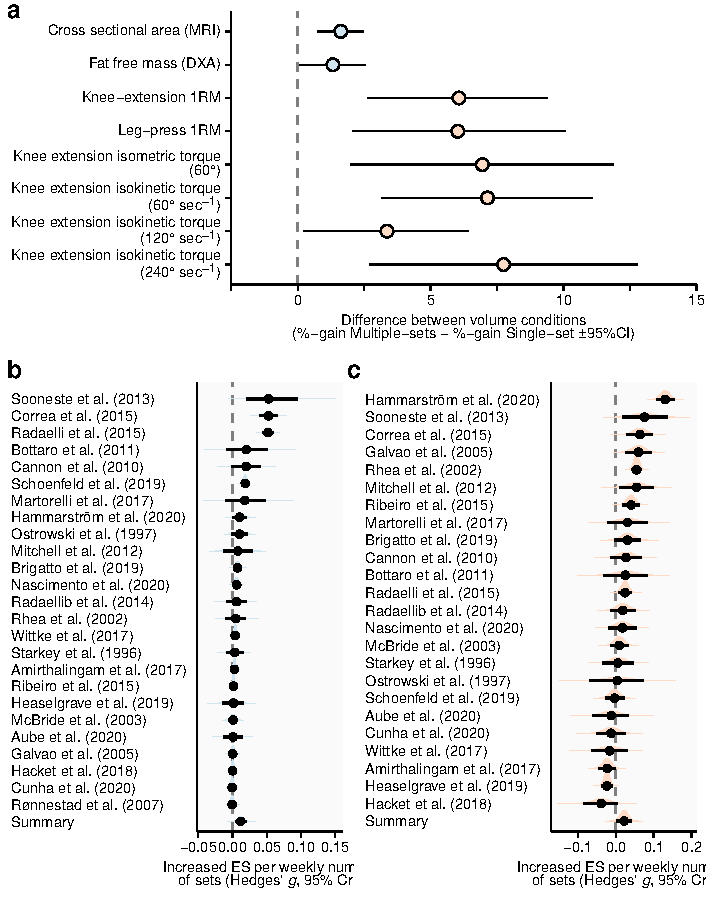
\includegraphics{thesis_files/figure-latex/comb-fig-s1-1} 

}

\caption[Differences in training induced changes to muscle mass and strength measures between volume conditions in Study I]{Differences in training induced relative changes in muscle mass and strength measures. Estimates are derived from ANCOVA models controling for baseline values and sex.}\label{fig:comb-fig-s1}
\end{figure}
\hypertarget{acute-effects-of-diffrent-training-volume-on-determinants-of-muscle-protein-synthesis}{%
\section{Acute effects of diffrent training volume on determinants of muscle protein synthesis}\label{acute-effects-of-diffrent-training-volume-on-determinants-of-muscle-protein-synthesis}}

Higher volume of acute resistance exercise led to increased phosphorylation of S6K1, ribosomal protein S6 and mTOR. These phosphorylation sites are indicative of activity along the mTORC1 pathway but mechanistic studies show that multiple sites exists for signal redundancy
Inhibiting mTOR by Torin1 after electrically stimulated muscle contractions still led to S6K1 phsophorylation

Regardless of upstream paralell signaling patterns the present result confirm volume dependency in a pathway controlling protein synthesis and ribosome biogenesis.

A limitation in the present study is that the limited panel of antibodies and time-points used to capture volume

\hypertarget{general-discussion}{%
\chapter{General Discussion}\label{general-discussion}}

Constant volume protocols with higher volume within a tolerable range produces favorable adaptations regarding muscle hypertrophy.

\hypertarget{conclusion}{%
\chapter*{Conclusion}\label{conclusion}}
\addcontentsline{toc}{chapter}{Conclusion}

If we don't want Conclusion to have a chapter number next to it, we can add the \texttt{\{-\}} attribute.

\textbf{More info}

And here's some other random info: the first paragraph after a chapter title or section head \emph{shouldn't be} indented, because indents are to tell the reader that you're starting a new paragraph. Since that's obvious after a chapter or section title, proper typesetting doesn't add an indent there.

\backmatter

\hypertarget{references}{%
\chapter*{References}\label{references}}
\addcontentsline{toc}{chapter}{References}

\markboth{References}{References}

\noindent

\setlength{\parindent}{-0.20in}
\setlength{\leftskip}{0.20in}
\setlength{\parskip}{8pt}

\hypertarget{refs}{}
\leavevmode\hypertarget{ref-RN2512}{}%
1. Li R, Xia J, Zhang XI, Gathirua-Mwangi WG, Guo J, Li Y, et al. Associations of muscle mass and strength with all-cause mortality among us older adults. Medicine and science in sports and exercise {[}Internet{]}. 2018;50(3):458--67.

\leavevmode\hypertarget{ref-RN2513}{}%
2. Fukasawa H, Kaneko M, Niwa H, Matsuyama T, Yasuda H, Kumagai H, et al. Lower thigh muscle mass is associated with all-cause and cardiovascular mortality in elderly hemodialysis patients. European Journal of Clinical Nutrition {[}Internet{]}. 2017;71(1):64--9.

\leavevmode\hypertarget{ref-RN2514}{}%
3. Miyake H, Kanazawa I, Tanaka KI, Sugimoto T. Low skeletal muscle mass is associated with the risk of all-cause mortality in patients with type 2 diabetes mellitus. Ther Adv Endocrinol Metab {[}Internet{]}. 2019;10:2042018819842971.

\leavevmode\hypertarget{ref-RN2376}{}%
4. Ruiz JR, Sui X, Lobelo F, Morrow J James R., Jackson AW, Sjöström M, et al. Association between muscular strength and mortality in men: Prospective cohort study. BMJ (Clinical research ed) {[}Internet{]}. 2008;337(7661):a439--9.

\leavevmode\hypertarget{ref-RN2515}{}%
5. Szulc P, Munoz F, Marchand F, Chapurlat R, Delmas PD. Rapid loss of appendicular skeletal muscle mass is associated with higher all-cause mortality in older men: The prospective minos study. Am J Clin Nutr {[}Internet{]}. 2010;91(5):1227--36.

\leavevmode\hypertarget{ref-RN2516}{}%
6. Abramowitz MK, Hall CB, Amodu A, Sharma D, Androga L, Hawkins M. Muscle mass, bmi, and mortality among adults in the united states: A population-based cohort study. PLoS One. 2018;13(4):e0194697.

\leavevmode\hypertarget{ref-RN2517}{}%
7. Janssen I, Heymsfield SB, Ross R. Low relative skeletal muscle mass (sarcopenia) in older persons is associated with functional impairment and physical disability. J Am Geriatr Soc {[}Internet{]}. 2002;50(5):889--96.

\leavevmode\hypertarget{ref-RN2532}{}%
8. Sousa AS, Guerra RS, Fonseca I, Pichel F, Ferreira S, Amaral TF. Financial impact of sarcopenia on hospitalization costs. Eur J Clin Nutr {[}Internet{]}. 2016;70(9):1046--51.

\leavevmode\hypertarget{ref-RN2184}{}%
9. Pinedo-Villanueva R, Westbury LD, Syddall HE, Sanchez-Santos MT, Dennison EM, Robinson SM, et al. Health care costs associated with muscle weakness: A uk population-based estimate. Calcif Tissue Int {[}Internet{]}. 2019;104(2):137--44.

\leavevmode\hypertarget{ref-RN763}{}%
10. Wolfe RR. The underappreciated role of muscle in health and disease. Am J Clin Nutr {[}Internet{]}. 2006;84(3):475--82.

\leavevmode\hypertarget{ref-RN2526}{}%
11. Arden NK, Spector TD. Genetic influences on muscle strength, lean body mass, and bone mineral density: A twin study. Journal of Bone and Mineral Research {[}Internet{]}. 1997;12(12):2076--81.

\leavevmode\hypertarget{ref-RN2527}{}%
12. Roth SM. Genetic aspects of skeletal muscle strength and mass with relevance to sarcopenia. BoneKEy reports {[}Internet{]}. 2012;1:58--8.

\leavevmode\hypertarget{ref-RN1741}{}%
13. Ahtiainen JP, Walker S, Peltonen H, Holviala J, Sillanpaa E, Karavirta L, et al. Heterogeneity in resistance training-induced muscle strength and mass responses in men and women of different ages. Age (Dordr) {[}Internet{]}. 2016;38(1):10.

\leavevmode\hypertarget{ref-RN2534}{}%
14. Grgic J, Garofolini A, Orazem J, Sabol F, Schoenfeld BJ, Pedisic Z. Effects of resistance training on muscle size and strength in very elderly adults: A systematic review and meta-analysis of randomized controlled trials. Sports Med {[}Internet{]}. 2020;

\leavevmode\hypertarget{ref-RN2536}{}%
15. Faigenbaum AD, Myer GD. Resistance training among young athletes: Safety, efficacy and injury prevention effects. British Journal of Sports Medicine {[}Internet{]}. 2010;44(1):56.

\leavevmode\hypertarget{ref-RN1}{}%
16. Ratamess N, Alvar BA, Evetoch TK, Housh TJ, Kibler B, Kraemer WJ, et al. American college of sports medicine position stand. Progression models in resistance training for healthy adults. Med Sci Sports Exerc {[}Internet{]}. 2009;41(3):687--708.

\leavevmode\hypertarget{ref-RN798}{}%
17. Bird SP, Tarpenning KM, Marino FE. Designing resistance training programmes to enhance muscular fitness: A review of the acute programme variables. Sports Med {[}Internet{]}. 2005;35(10):841--51.

\leavevmode\hypertarget{ref-RN2538}{}%
18. Feigenbaum MS, Pollock ML. Prescription of resistance training for health and disease. Med Sci Sports Exerc. 1999;31(1):38--45.

\leavevmode\hypertarget{ref-RN791}{}%
19. Burd NA, Holwerda AM, Selby KC, West DW, Staples AW, Cain NE, et al. Resistance exercise volume affects myofibrillar protein synthesis and anabolic signalling molecule phosphorylation in young men. J Physiol {[}Internet{]}. 2010;588(Pt 16):3119--30.

\leavevmode\hypertarget{ref-RN784}{}%
20. Terzis G, Spengos K, Mascher H, Georgiadis G, Manta P, Blomstrand E. The degree of p70 s6k and s6 phosphorylation in human skeletal muscle in response to resistance exercise depends on the training volume. Eur J Appl Physiol {[}Internet{]}. 2010;110(4):835--43.

\leavevmode\hypertarget{ref-RN1837}{}%
21. Ahtiainen JP, Walker S, Silvennoinen M, Kyrolainen H, Nindl BC, Hakkinen K, et al. Exercise type and volume alter signaling pathways regulating skeletal muscle glucose uptake and protein synthesis. Eur J Appl Physiol. 2015;115(9):1835--45.

\leavevmode\hypertarget{ref-RN793}{}%
22. Krieger JW. Single versus multiple sets of resistance exercise: A meta-regression. J Strength Cond Res {[}Internet{]}. 2009;23(6):1890--901.

\leavevmode\hypertarget{ref-RN789}{}%
23. Krieger JW. Single vs. Multiple sets of resistance exercise for muscle hypertrophy: A meta-analysis. J Strength Cond Res {[}Internet{]}. 2010;24(4):1150--9.

\leavevmode\hypertarget{ref-RN1767}{}%
24. Schoenfeld BJ, Ogborn D, Krieger JW. Dose-response relationship between weekly resistance training volume and increases in muscle mass: A systematic review and meta-analysis. J Sports Sci {[}Internet{]}. 2016;1--10.

\leavevmode\hypertarget{ref-RN2063}{}%
25. Choi J, Lee M, Lee JK, Kang D, Choi JY. Correlates associated with participation in physical activity among adults: A systematic review of reviews and update. BMC Public Health {[}Internet{]}. 2017;17(1):356.

\leavevmode\hypertarget{ref-RN794}{}%
26. Carpinelli RN, Otto RM. Strength training. Single versus multiple sets. Sports Med {[}Internet{]}. 1998;26(2):73--84.

\leavevmode\hypertarget{ref-RN2547}{}%
27. Pickering C, Kiely J. Do non-responders to exercise exist---and if so, what should we do about them? Sports Medicine {[}Internet{]}. 2019;49(1):1--7.

\leavevmode\hypertarget{ref-RN1476}{}%
28. Berger R. Effect of varied weight training-programs on strength. Research Quarterly {[}Internet{]}. 1962;33(2):168--81.

\leavevmode\hypertarget{ref-RN2568}{}%
29. Carpinelli RN. Berger in retrospect: Effect of varied weight training programmes on strength. British Journal of Sports Medicine {[}Internet{]}. 2002;36(5):319.

\leavevmode\hypertarget{ref-RN2201}{}%
30. Carpinelli RN. Science versus opinion. British journal of sports medicine {[}Internet{]}. 2004;38(2):240--2.

\leavevmode\hypertarget{ref-RN2523}{}%
31. Newman AB, Kupelian V, Visser M, Simonsick EM, Goodpaster BH, Kritchevsky SB, et al. Strength, but not muscle mass, is associated with mortality in the health, aging and body composition study cohort. J Gerontol A Biol Sci Med Sci {[}Internet{]}. 2006;61(1):72--7.

\leavevmode\hypertarget{ref-RN2492}{}%
32. Ralston GW, Kilgore L, Wyatt FB, Baker JS. The effect of weekly set volume on strength gain: A meta-analysis. Sports Med {[}Internet{]}. 2017;47(12):2585--601.

\leavevmode\hypertarget{ref-RN1612}{}%
33. Schoenfeld BJ, Ratamess NA, Peterson MD, Contreras B, Sonmez GT, Alvar BA. Effects of different volume-equated resistance training loading strategies on muscular adaptations in well-trained men. J Strength Cond Res {[}Internet{]}. 2014;28(10):2909--18.

\leavevmode\hypertarget{ref-RN1049}{}%
34. Goodman CA. The role of mTORC1 in regulating protein synthesis and skeletal muscle mass in response to various mechanical stimuli. Rev Physiol Biochem Pharmacol {[}Internet{]}. 2014;

\leavevmode\hypertarget{ref-RN782}{}%
35. Bodine SC, Stitt TN, Gonzalez M, Kline WO, Stover GL, Bauerlein R, et al. Akt/mTOR pathway is a crucial regulator of skeletal muscle hypertrophy and can prevent muscle atrophy in vivo. Nat Cell Biol {[}Internet{]}. 2001;3(11):1014--9.

\leavevmode\hypertarget{ref-RN780}{}%
36. Drummond MJ, Fry CS, Glynn EL, Dreyer HC, Dhanani S, Timmerman KL, et al. Rapamycin administration in humans blocks the contraction-induced increase in skeletal muscle protein synthesis. J Physiol {[}Internet{]}. 2009;587(Pt 7):1535--46.

\leavevmode\hypertarget{ref-RN785}{}%
37. Terzis G, Georgiadis G, Stratakos G, Vogiatzis I, Kavouras S, Manta P, et al. Resistance exercise-induced increase in muscle mass correlates with p70S6 kinase phosphorylation in human subjects. Eur J Appl Physiol {[}Internet{]}. 2008;102(2):145--52.

\leavevmode\hypertarget{ref-RN866}{}%
38. Baar K, Esser K. Phosphorylation of p70(S6k) correlates with increased skeletal muscle mass following resistance exercise. Am J Physiol {[}Internet{]}. 1999;276(1 Pt 1):C120--7.

\leavevmode\hypertarget{ref-RN2548}{}%
39. World medical association declaration of helsinki: Ethical principles for medical research involving human subjects. Jama {[}Internet{]}. 2013;310(20):2191--4.

\leavevmode\hypertarget{ref-RN2541}{}%
40. Tavoian D, Ampomah K, Amano S, Law TD, Clark BC. Changes in dxa-derived lean mass and mri-derived cross-sectional area of the thigh are modestly associated. Scientific Reports {[}Internet{]}. 2019;9(1):10028.

\leavevmode\hypertarget{ref-RN824}{}%
41. Hayot M, Michaud A, Koechlin C, Caron MA, Leblanc P, Prefaut C, et al. Skeletal muscle microbiopsy: A validation study of a minimally invasive technique. Eur Respir J {[}Internet{]}. 2005;25(3):431--40.

\leavevmode\hypertarget{ref-RN2549}{}%
42. Ekblom B. The muscle biopsy technique. Historical and methodological considerations. Scand J Med Sci Sports {[}Internet{]}. 2017;27(5):458--61.

\leavevmode\hypertarget{ref-RN2553}{}%
43. Bonafiglia JT, Islam H, Preobrazenski N, Drouin P, Ma A, Gerhart A, et al. A comparison of pain responses, hemodynamic reactivity and fibre type composition between bergström and microbiopsy skeletal muscle biopsies. Current Research in Physiology {[}Internet{]}. 2020;3:1--10.

\leavevmode\hypertarget{ref-RN2552}{}%
44. Hughes MC, Ramos SV, Turnbull PC, Nejatbakhsh A, Baechler BL, Tahmasebi H, et al. Mitochondrial bioenergetics and fiber type assessments in microbiopsy vs. Bergstrom percutaneous sampling of human skeletal muscle. Frontiers in Physiology {[}Internet{]}. 2015;6(360).

\leavevmode\hypertarget{ref-RN874}{}%
45. Blomstrand E, Ekblom B. The needle biopsy technique for fibre type determination in human skeletal muscle--a methodological study. Acta Physiol Scand {[}Internet{]}. 1982;116(4):437--42.

\leavevmode\hypertarget{ref-RN2007}{}%
46. Bland M. An introduction to medical statistics. Fourth edition. Oxford ; Oxford University Press; 2015. (Oxford medical publications).


% Index?

\end{document}
